\section{Minimization and comparison of labeled transition systems}
\label{sec:bisimulation}

Bisimulation equivalence (bisimilarity) \cite{Park} is a binary relation between labeled transition systems which associates systems that can simulate each other's behaviour in a stepwise manner, enabling comparison of different transition systems \cite{ModelChecking}. An alternative perspective is to consider the bisimulation equivalence as a relation between states of a single labeled transition system, providing means for construction of smaller models of the system using the quotient transition system under such a relation \cite{ModelChecking}.

TMACS implements both options: reducing the size of the state space of a given labeled transition system and checking the equivalence of two labeled transition systems, using two behavioral equivalence relations: strong bisimilarity and observational equivalence (weak bisimilarity).

\subsection{Minimization of a labeled transition system modulo strong bisimilarity}
The process of reducing the size of the state space of a labeled transition system $A=\left(S, Act, \rightarrow, s, F \right)$ in TMACS was implemented using an approach which consists of two steps:
\begin{enumerate}
\item Computing strong bisimulation equivalence (strong bisimilarity) for the labeled transition system;
\item Minimizing the labeled transition system to its canonical form using the strong bisimilarity obtained in the first step;
\end{enumerate}

Two different methods were used for computing the strong bisimulation equivalence: the so called naive method and a more efficient 
method due to Fernandez, both of which afterwards serve as minimization procedures.

The naive algorithm for computing strong bisimulation over finite labeled transition systems stems directly from the theory of partially ordered sets and lattices \cite{ReactiveSystems} underlying Tarski's classic fixed point theorem \cite{Tarsky}. This algorithm has time complexity of $O(mn)$ for a labeled transition system with \emph{m} transitions and \emph{n} states. Its implementation in TMACS takes as an input a labeled transition system in Aldebaran format, and generates the corresponding labeled graph as a list of nodes representing the states which use the following data structure:
\begin{itemize}
	\item $S_p=\{(a, q)\hspace{1mm}|\hspace{1mm} p\stackrel{a}{\rightarrow}q, \hspace{1mm} p,q\in \mathit{S}, \hspace{1mm} a\in \mathit{Act}\}$ - set of pairs $(a, q)$ for state $p$ where $a$ is an outgoing action for $p$ and $q$ is a state
	reachable from $p$ with action $a$
\end{itemize}
The algorithm then computes the strong bisimulation equivalence and outputs it as pairs of bisimilar states $L = \left\{\left(p,q\right)|\hspace{1mm}\hspace{1mm} p\sim q, \hspace{1mm}p,q\in \mathit{S}\right\}$.
%\begin{equation*}
%	L = \left\{\left(p,q\right)|\hspace{1mm}\hspace{1mm} p\sim q, \hspace{1mm}p,q\in \mathit{S}\right\}
%\end{equation*}

The algorithm due to Fernandez exploits the idea of the relationship between strong bisimulation equivalence 
and the relational coarsest partition problem \cite{KanellakisSmolka} solved by Paige and Tarjan in $O(m \log n)$ time \cite{PaigeTarjan}. Fernandez's adaptation of the algorithm of Paige-Tarjan has the same complexity as the original one, major difference being that a refinement step is made with only one element of $Act$ in the original one. Our implementation of the algorithm takes as an input a labeled transition system in Aldebaran format, generates a labeled graph and then partitions the labeled graph into its coarsest blocks where each block represents a set of bisimilar states. To define graph states 
and transitions the following terminology is used represented by suitable data structures: 
\begin{itemize}
	\item $T_a[p]=\{q\}$ - an $a$-transition from state $p$ to state $q$
	\item $T_a{}^{-1}[q]=\{p\}$ - an inverse $a$-transition from state $q$ to state $p$
	\item $T_a{}^{-1}[B]=\cup \left\{T_a{}^{-1}[q],q\in B\right\}$ - inverse transition for block $B$ and action $a$
	\item $W$ - set of sets called splitters that are being used to split the partition
	\item infoB$(a, p)$ - info map for block $B$, state $p$ and action $a$
\end{itemize}

The algorithm of Fernandez outputs the strong bisimulation equivalence relation over $\mathit{Proc}$ as a partition $P = \left\{B_{i}\hspace{1mm}|\hspace{1mm} p\sim q,\hspace{1mm} \forall p,q\in B_{i}, i=\overline{1,n} \right\}$ where $B_{i}$, $i=\overline{1,n}$, represent its equivalence classes.

%The algorithm of Fernandez outputs the strong bisimulation equivalence relation over $\mathit{Proc}$ as a partition %$P=\left\{B_{1},...,B_{n}\right\}$ where $B_{i}$, $i=\overline{1,n}$, represent its equivalence classes: $P = %\left\{B_{i}\hspace{1mm}|\hspace{1mm} p\sim q,\hspace{1mm} \forall p,q\in B_{i}, i=\overline{1,n} \right\}$.
%\begin{equation*}
%	P = \left\{B_{i}\hspace{1mm}|\hspace{1mm} p\sim q,\hspace{1mm} \forall p,q\in B_{i}, i=\overline{1,n} \right\}
%\end{equation*}

Having computed the strong bisimulation equivalence, the next step in the reduction of the state space of the labeled transition system uses the bisimulation equivalence obtained in the first step in order to minimize the labeled graph. This reduction is implemented as follows:
\begin{enumerate}
	\item All states in a bisimilar equivalence class $B_{i}$ are merged into one single state $k=\bigcup p_{j}$, for $p_{j}\in B_{i}$;
	\item All incoming transitions $r \stackrel{a}{\rightarrow} p_{j}$, for $p_{j}\in B_{i}$, are replaced by transitions $r \stackrel{a}{\rightarrow} k$;
	\item All outgoing transitions $p_{j} \stackrel{a}{\rightarrow} t$, for $p_{j}\in B_{i}$, are replaced by transitions $k \stackrel{a}{\rightarrow} t$;
	\item The duplicate transitions are not taken into consideration.
\end{enumerate}
The procedure is repeated for all equivalence classes $B_{i}$, $i\in \overline{1,n}$.

\subsection{Minimization of a labeled transition system modulo weak bisimilarity}
The minimization of a labeled transition system modulo weak bisimilarity is reduced to the problem of minimization modulo strong bisimilarity, using a technique called saturation. Saturation first precomputes the weak transition relation and then constructs a new pair of finite processes whose original transitions are replaced by the weak transitions \cite{ReactiveSystems}. 

The algorithm for saturation in TMACS is implemented as follows: 
\begin{enumerate}
\item For every ${p\in \mathit{S}}$, the set of all transitions $T$ of a labeled system with $m$ transitions and $n$ states is partitioned in ${2n}$ sets with ${T_{\mathit{\tau p}}=\left\{\left(p,\tau,q\right)| \left(p,\tau,q\right)\right\}}$ and ${T_{ap}=\left\{\left(p,a,q\right)| \left(p,a,q\right)\wedge a\neq\tau\right\}}$. 
%\begin{equation*}
%	\begin{array}{lcl}
% 		{T_{\mathit{\tau p}}=\left\{\left(p,\tau,q\right)| \left(p,\tau,q\right)\right\}}, \text{and}\\
%    {T_{ap}=\left\{\left(p,a,q\right)| \left(p,a,q\right)\wedge a\neq\tau\right\}}
%  \end{array}
%\end{equation*} 
\\
Then the family of sets ${T^{'}_{\tau p}}$ is iteratively constructed as:
\begin{equation*}
	\begin{array}{lcl}
		{T^{0}_{\mathit{\tau p}}=T_{\mathit{\tau p}}\cup\left\{\left(p,\tau,p\right)\right\}},\\
		{T^{i}_{\mathit{\tau p}}=T^{i-1}_{\mathit{\tau p}}\cup\left\{\left(p,\tau,q'\right)|\left(\exists q\in \mathit{S}\right)\left(p,\tau,q\right)\in T^{i-1}_{\mathit{\tau p}}\wedge\left(q,\tau,q'\right)\in T_{\mathit{\tau q}}\right\}}, \text{and} \\
		{T^{'}_{\mathit{\tau p}}=T^{n}_{\mathit{\tau p}}}
	\end{array}
\end{equation*}

With this step a reflexive, transitive closure of $\tau$ is constructed:
\begin{equation*}
	{T^{*}_{\tau}=\bigcup_{p\in \mathit{S}}T^{'}_{\tau p}=\left\{\left(p,\tau,q\right)|\hspace{1mm}p\left(\stackrel{\tau}{\rightarrow}\right)^{*}q\right\}}
\end{equation*}

\item Next, $T'_{s}=\bigcup_{p\in \mathit{S}}T'_{ap}=\left\{\left(p,a,q\right)|\left(\exists q'\in \mathit{S}\right)\left(p,a,q'\right)\in T\wedge q'\left(\stackrel{\tau}{\rightarrow}\right)^{*}q\right\}$ is constructed as follows:
%\begin{equation*}\label{eq:tap}
%		T'_{s}=\bigcup_{p\in \mathit{S}}T'_{ap}=\left\{\left(p,a,q\right)|\left(\exists q'\in \mathit{S}\right)\left(p,a,q'\right)\in T\wedge q'\left(\stackrel{\tau}{\rightarrow}\right)^{*}q\right\}
%\end{equation*}
%as follows:
\begin{equation*}
	\begin{array}{lcl}
		T^{0}_{sp}=T_{sp},\\
		T^{i}_{sp}=T^{i-1}_{sp}\cup \left\{\left(p,a,q'\right)|\left(\exists q\in \mathit{S}\right)\left(p,a,q\right)\in T^{i-1}_{sp}\wedge \left(q,\tau,q'\right)\in T^{i-1}_{\tau q}\right\} \text{and} \\
		T'_{sp}=T^{n|\mathit{Act}|}_{sp}
	\end{array}
\end{equation*}

\item $T'=\bigcup_{p\in \mathit{S}}\left(T^{'}_{\mathit{\tau p}}\cup T'_{sp}\right)$ is partitioned again for every $p\in \mathit{S}$, defined by the destination in the transition triple, with $T^{*}_{\mathit{\tau q}}=\left\{\left(p,\tau,q\right)|\left(p,\tau,q\right)\in T'\right\}$ and $T_{dq}=\left\{\left(p,a,q\right)|\hspace{1mm}\left(p,a,q\right)\in T' a\neq\tau\right\}$.
%\begin{equation*}
%	\begin{array}{lcl}
%		T^{*}_{\mathit{\tau q}}=\left\{\left(p,\tau,q\right)|\left(p,\tau,q\right)\in T'\right\}, \text{and}\\
%		T_{dq}=\left\{\left(p,a,q\right)|\hspace{1mm}\left(p,a,q\right)\in T' a\neq\tau\right\}				    
%	\end{array}
%\end{equation*}
\\
Then the family of sets ${T^{*}_{dq}}$ is iteratively constructed as:
\begin{equation*}
	\begin{array}{lcl}
		T^{0}_{dq}=T_{dq},\\
		T^{i}_{dq}=T^{i-1}_{dq}\cup\left\{\left(p',a,q\right)|\left(\exists p\in \mathit{S}\right)\left(p,a,q\right)\in T^{i-1}_{dq}\wedge\left(p',\tau,p\right)\in T^{*}_{\tau p}\right\} \text{, and}\\
		T^{*}_{dq}=T^{n|\mathit{Act}|}_{dq}
	\end{array}
\end{equation*}
\end{enumerate}

Finally the saturated labeled transition system now is:
\begin{align*}
	T^{*} &=\bigcup_{p\in \mathit{S}}\left(T^{*}_{\mathit{\tau p}}\cup T^{*}_{dp}\right)=\\
	&=\left(\stackrel{\tau}{\rightarrow}\right)^{*}\cup\left\{\left(p,a,q\right)|\hspace{1mm}a\neq\tau\wedge\left(\exists p',q'\in S\right)\hspace{1mm} p\left(\stackrel{\tau}{\rightarrow}\right)^{*}p'\stackrel{a}{\rightarrow}q'\left(\stackrel{\tau}{\rightarrow}\right)^{*}q\right\}
\end{align*}

An illustration of a saturated labeled transition system before and after applying the saturation technique is given on Fig.~\ref{fig:saturation_example}:
%\\*
%\begin{figure}[h]
%\centering
%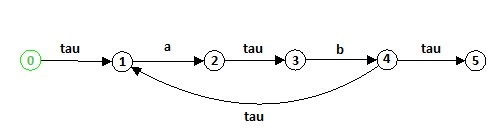
\includegraphics[width=4.0in]{saturation3}
%\caption{Example of a labeled graph before saturation}
%\label{fig:saturation3}
%\end{figure}
%\begin{figure}[h]
%\centering
%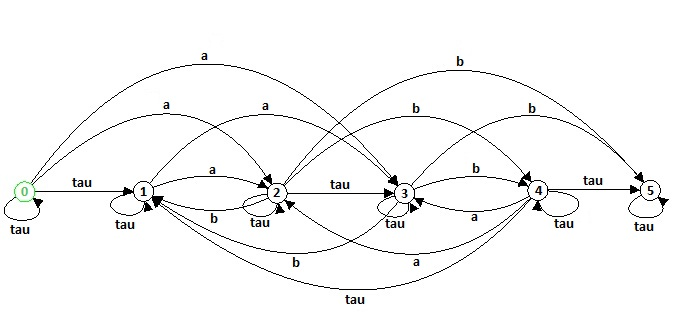
\includegraphics[width=4.5in]{saturation2}
%\caption{The labeled graph from Fig.~\ref{fig:saturation3} after saturation}
%\label{fig:saturation2}
%\end{figure}

%\begin{figure}[h]
%\begin{left}$
%\begin{array}{cc}
%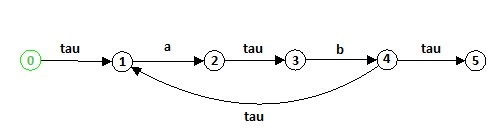
\includegraphics[width=3.0in]{saturation3.jpg} 
%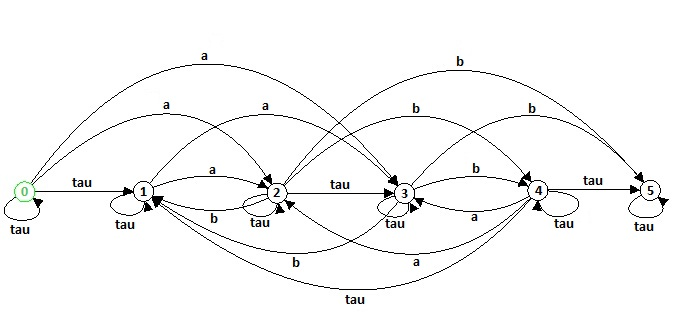
\includegraphics[width=3.5in]{saturation2.jpg}
%\end{array}$
%\end{center}
%\caption{my caption}
%\end{figure}

%\begin{figure}[h]
%\centering
%\subfloat{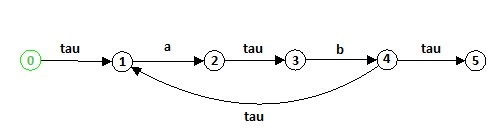
\includegraphics[width=4in]{saturation3.jpg}} \\
%\subfloat{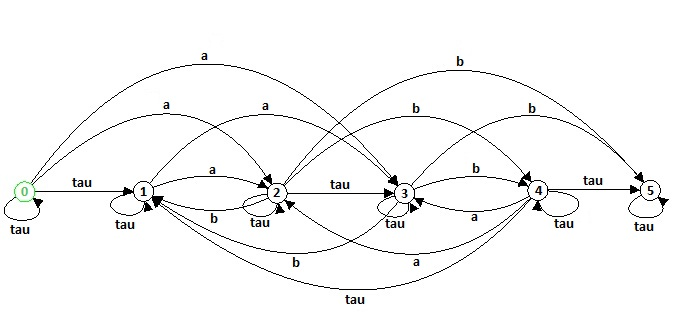
\includegraphics[width=4in]{saturation2.jpg}}
%\caption{Example of a labeled graph before and after saturation}
%\label{fig:saturation}
%\end{figure}

\begin{figure}[h]
\centering
\subfigure[The labeled graph before saturation]{
   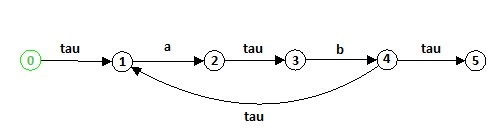
\includegraphics[width=3.5in]{saturation3}
   \label{fig:lts_before}
 }
 \subfigure[The labeled graph after saturation]{
   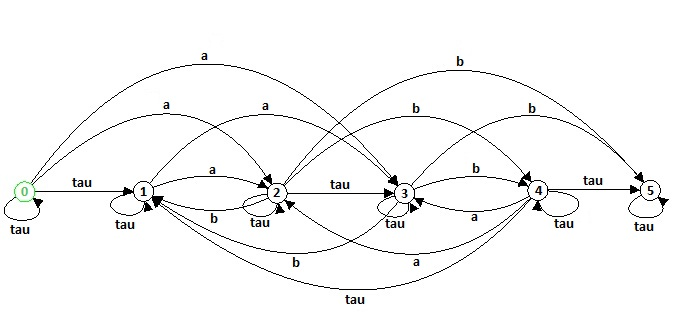
\includegraphics[width=4.2in]{saturation2}
   \label{fig:lts_after}
 }
\caption{Example of a labeled graph before and after applying the saturation technique}
\label{fig:saturation_example}
\end{figure}

Once the saturation algorithm is run and the original labeled transition system is saturated, the computation of weak bisimilarity amounts to computing strong bisimilarity over the saturated system. Afterwards, the process of minimization of the original system is the same as the process of minimization modulo strong bisimilarity applied on the saturated system.

\subsection{Comparison of two labeled transition systems modulo strong bisimilarity}
The idea for the implementation of the equivalence checking of two labeled transition systems modulo strong bisimilarity was based on the following fact: Two labelled transition systems are (strongly) bisimilar iff their initial states are bisimilar \cite{ModellingAndAnalysis}. That means that in order to check whether two labeled transition systems are bisimilar it is enough to check whether their initial states are bisimilar. This can be done using the following approach:
\begin{enumerate}
	\item The two labeled transition systems are merged into a single transition system
	\item An algorithm for computing the strong bisimilarity is applied to the merged system
	\item A check is performed to see if the initial states belong to the same bisimulation equivalence class
\end{enumerate}

\subsection{Comparison of two  labeled transition systems modulo weak bisimilarity}
The comparison of two labeled transition systems modulo weak bisimilariy amounts to checking strong bisimilarity over the saturated labeled transition systems \cite{ReactiveSystems}. In another words, two labeled transition systems are weakly bisimilar iff their saturated labeled transition systems are strongly bisimilar. Following this fact, we implemented the comparison of two labeled transition systems modulo weak bisimilarity by applying the saturation algorithm over the original labeled graphs in order to obtain their saturated labeled graphs, after which the process of comparison of the saturated labeled transition systems modulo strong bisimilarity was applied as described above.